\documentclass[final]{beamer}



% global default settings
\usepackage[orientation=landscape, scale=0.6, size=custom, height=60.96, width=91.44, debug]{beamerposter}
\usetheme{confposter}
	\setbeamercolor{block title}{fg=cardinalred, bg=white}
	\setbeamercolor{block body}{fg=black, bg=white}
	\setbeamercolor{block alerted title}{fg=white, bg=cardinalred}
	\setbeamercolor{block alerted body}{fg=Black, bg=cloud}
\usepackage[font=small,labelfont=bf]{caption}
\captionsetup[figure]{labelformat=simple}
\captionsetup[table]{labelformat=simple}

\usepackage{tabularx}
\newcolumntype{C}[1]{>{\centering\arraybackslash}p{#1}}
\usepackage{wrapfig}


% layout
% You can set your column widths, spacings, etc. here
% \setlength{\paperwidth}{36in}
% \setlength{\paperheight}{24in}
\newlength{\sepwid}
\setlength{\sepwid}{0.01\paperwidth}
\newlength{\firstcolwid}
\setlength{\firstcolwid}{0.18\paperwidth}
\newlength{\secondcolwid}
\setlength{\secondcolwid}{0.27\paperwidth}
\newlength{\thirdcolwid}
\setlength{\thirdcolwid}{0.27\paperwidth}
\newlength{\lastcolwid}
\setlength{\lastcolwid}{0.23\paperwidth}
\setlength{\topmargin}{-0.5in}

\addtobeamertemplate{block end}{}{\vspace*{1em}}
\addtobeamertemplate{block alerted end}{}{\vspace*{1em}}

% indentation needs to be set-up manually
% (beamer ignores indentations by default)
\makeatletter \addtobeamertemplate{block begin}{}{\setlength{\parindent}{1cm}\@afterindentfalse\@afterheading} \makeatletter

\usepackage[english]{babel}
\usepackage{blindtext}
\usepackage[utf8]{inputenc}
\usepackage{amsmath, amsthm, amssymb, latexsym}
% \usepackage[justification=centering,labelformat=empty]{caption}
% \captionsetup{font={rm}}
\usepackage{graphicx}
% \usepackage{moresize}
\usepackage{fix-cm}
\newcommand{\HUGE}{\fontsize{55}{60}\selectfont}
% \makeatletter
% \newcommand\HUGE{\@setfontsize\Huge{}{80}}
% \makeatother  
\usepackage{url}
\usepackage{tikz}
\usepackage{units}
\usepackage{changepage}
\usepackage{subcaption}
\usepackage{physics}
\usepackage{empheq}
\usepackage{tcolorbox}
\usepackage{natbib}

% make bibliography entries smaller
% \renewcommand\bibfont{\scriptsize}
% If you have more than one page of references, you want to tell beamer
% to put the continuation section label from the second slide onwards
\setbeamertemplate{frametitle continuation}[from second]
% Now get rid of all the colours
% (fancy colors in bibliography/reference is unnecessary...)
\setbeamercolor*{bibliography entry title}{fg=black}
\setbeamercolor*{bibliography entry author}{fg=black}
\setbeamercolor*{bibliography entry location}{fg=black}
\setbeamercolor*{bibliography entry note}{fg=black}
% and kill the abominable icon
\setbeamertemplate{bibliography item}{}

% Emphasize with Palo Alto Green
\newcommand{\emphg}[1]{{\color{paloalto}\textbf{#1}}}
% Emphasize with Cardinal Red
\newcommand{\emphr}[1]{{\color{cardinalred}\textbf{#1}}}




\title{
	\HUGE\color{cardinalred}
	Stanford University
}
\author{
	\large{
	Sanha Cheong,
	Sanha Cheong\textsuperscript{$*$},
	Sanha Cheong\textsuperscript{$\dagger$}		\\
	\href{emailto:sanha@stanford.edu}{\texttt{sanha@stanford.edu}},
	\href{emailto:sanha@stanford.edu}{\texttt{sanha@stanford.edu}},
	\href{emailto:sanha@stanford.edu}{\texttt{sanha@stanford.edu}}
	}
}
\institute{
	\large{
	Department of Physics, Stanford University	\\
	SLAC National Accelerator Laboratory
	}
}
\date{\today}


\begin{document}
\addtobeamertemplate{headline}{} 
{
	\begin{tikzpicture}[remember picture, overlay]
	% logo at top left corner
	\node [anchor=north west, inner sep=2cm]  at (current page.north west)
	{
\includegraphics[height=5.5cm]{./img/SUSig_Stack.eps}};
	\end{tikzpicture}
	\begin{tikzpicture}[remember picture, overlay]
	% logo at top right corner
     \node [anchor=north east, inner sep=2cm]  at (current page.north east)
     {
\includegraphics[height=5.5cm]{./img/SU_New_BlockStree_2color.eps}};
 \end{tikzpicture}}
\begin{frame}[t]



% Start your poster contents below the title

\begin{columns}[t]

\begin{column}{\sepwid}\end{column}

\begin{column}{\firstcolwid}

	\begin{alertblock}{\textbf{Structure}}
		
		This is an \emphr{example poster}.
		
		The \LaTeX \, code for this poster template is structured such that you place \emphg{\texttt{column}} environments within the main, overarching \emphg{\texttt{columns}} environment. Note that you should also set ``separation" columns to put spacing between columns. These column widths are set-up manually at the beginning of the document, near line 21.
		
		Within each \texttt{column}, you can put one or multiple \emphg{\texttt{block}} and/or \emphg{\texttt{alertblock}} environments. This one is an \texttt{alertblock}, and the one below is a regular \texttt{block}. A little unfortunate caveat is that the paragraphs are not automatically indented inside an \texttt{alertblock}. If you want consistent indenting, this has to be done manually:
		
		\hspace{1cm} like so, with the command \texttt{\textbackslash hspace\{1cm\}}. Paragraphs are indented automatically in regular \texttt{block} environments.
	\end{alertblock}
	
	\begin{block}{Emphasizing Texts}
		There are two main built-in ways to emphasize important texts, with two different colors: \emphr{Cardinal Red} with \texttt{\textbackslash emphr\{text\}} and \emphg{Palo Alto Green} with \texttt{\textbackslash emphg\{text\}}.
		
		These commands make the text boldfaced and color accordingly. (Note that this paragraph is indented by 1cm automatically, without explicit \texttt{\textbackslash hspace\{1cm\}} command.)
	\end{block}

\end{column}

\begin{column}{\sepwid}\end{column}

%\vspace{-1em}
\begin{column}[t]{\secondcolwid}
	\begin{block}{Figures \& Wrap-figures}
		
		You can of course add figures as you usually do in any \LaTeX \, document.
		
		\begin{figure}[H]
			\centering
			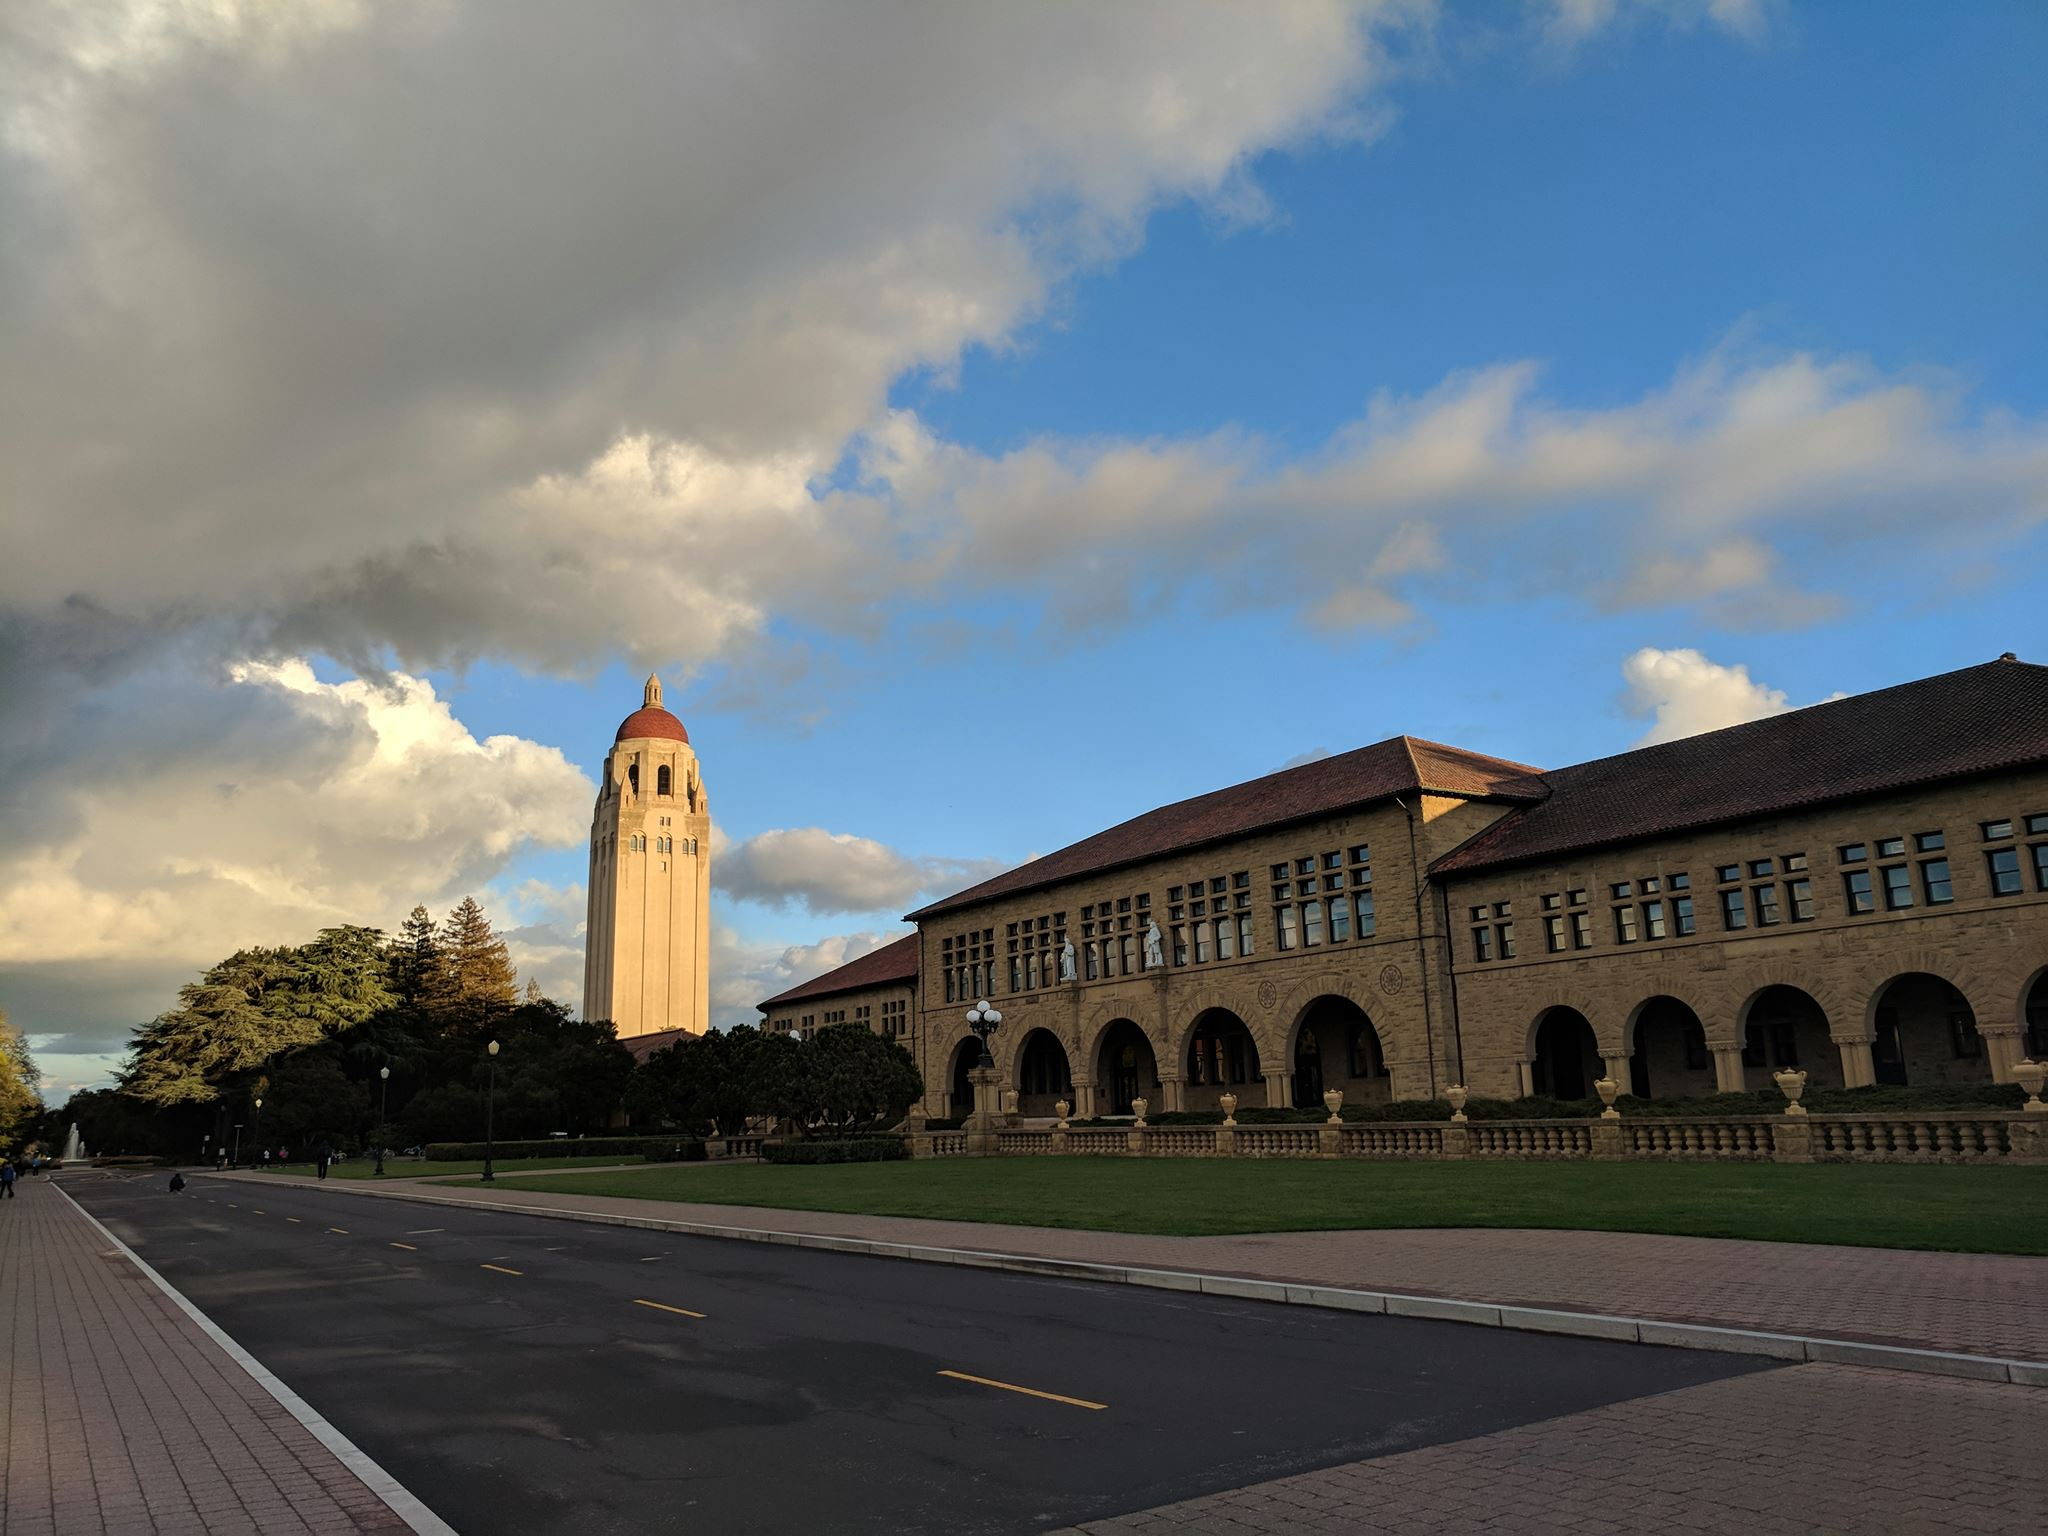
\includegraphics[height=4in]{./img/stanford_photo.jpg}
			\caption{A photo of Stanford main campus, taken by me}
			\label{fig:stanford_photo}
		\end{figure}
		
		You can also use the \texttt{wrapfigure} environment to insert a figure and wrap around it with text, but this requires some careful tuning of the widths and the sizes of your images and the text surrounding it. This can become \textit{very} tricky, but I have not found an easy alternative that works with \texttt{beamer} environment easily.

    	\begin{wrapfigure}{r}{14cm}
        	\vspace{0.5cm}
% 		\begin{figure}
        	
\includegraphics[height=4in]{./img/logo.jpg}
            \caption{Stanford University logo \cite{StanfordLogo}
            }
            \label{fig:stanford_logo}
        \end{wrapfigure}
% 		\end{figure}

		These are some random texts just to demonstrate how the paragraphs can wrap around the images you insert using \texttt{wrapfigure} environment. The wrapping works the best when your paragraph ends nicely at the (vertical) end of your image.
		
		Again, this can sometime become very tricky, so don't obsess yourself over it too much. It might sometimes be easier to paraphrase/re-word your text wrapping around, rather than to fiddle around with the \texttt{wrapfigure} alignment and width settings. I am going to make this paragraph just a little bit longer so that it ends nicely at the end of the logo image to the right.
        
        \begin{wrapfigure}{l}{8cm}
        	\centering
            
\includegraphics[width=8cm]{./img/SU_Seal_Red.png}
        	\caption{Stanford University official seal \cite{StanfordLogo}}
        	\label{fig:stanford_seal}
        \end{wrapfigure}
        
        Because the previous paragraph ended nicely at the end of Fig.~\ref{fig:stanford_logo}, this paragraph wraps smoothly around Fig.~\ref{fig:stanford_seal}, the image to our left.
        
        If you find an easier way of wrapping text around a figure in this beamer poster template, please leave a pull request on \emphg{\href{https://github.com/sanhacheong/stanford_beamer_poster}{the GitHub repository}} or leave me an \emphg{\href{mailto:sanha@stanford.edu}{email}}.

	\end{block}
	 
    
    
\end{column}

\begin{column}{\sepwid}\end{column}

\begin{column}[t]{\thirdcolwid}
	
	\begin{block}{Disclaimer \& License}
		
		Discalimer: This is \emphr{not an official template}, by any means supported or sponsored by Stanford University. This is made by me personally and shared for those at Stanford who need such a template or others who want to build their own templates based on this.
    
	    This file (and everything in the GitHub repository) is licensed under \emphg{the MIT License}.
	    
	    \begin{center}
	    	\textbf{MIT License}
	    	
	    	Copyright (c) 2018 Sanha Cheong
	    \end{center}
	    
	    Permission is hereby granted, free of charge, to any person obtaining a copy
	    of this software and associated documentation files (the "Software"), to deal
	    in the Software without restriction, including without limitation the rights
	    to use, copy, modify, merge, publish, distribute, sublicense, and/or sell
	    copies of the Software, and to permit persons to whom the Software is
	    furnished to do so, subject to the following conditions:
	    
	    The above copyright notice and this permission notice shall be included in all
	    copies or substantial portions of the Software.
	    
	    THE SOFTWARE IS PROVIDED "AS IS", WITHOUT WARRANTY OF ANY KIND, EXPRESS OR
	    IMPLIED, INCLUDING BUT NOT LIMITED TO THE WARRANTIES OF MERCHANTABILITY,
	    FITNESS FOR A PARTICULAR PURPOSE AND NONINFRINGEMENT. IN NO EVENT SHALL THE
	    AUTHORS OR COPYRIGHT HOLDERS BE LIABLE FOR ANY CLAIM, DAMAGES OR OTHER
	    LIABILITY, WHETHER IN AN ACTION OF CONTRACT, TORT OR OTHERWISE, ARISING FROM,
	    OUT OF OR IN CONNECTION WITH THE SOFTWARE OR THE USE OR OTHER DEALINGS IN THE
	    SOFTWARE.
	    
	    \vspace{1cm}
	    TL;DR: You can do whatever you want with this, as far as: \emphg{``The above copyright notice and this permission notice shall be included in all copies or substantial portions of the Software."}
	
	\end{block}
    
    \begin{block}{References}
		{\small
			\bibliographystyle{abbrv}
            %\bibliographystyle{acm}
			\bibliography{./bibliography}
		}
	\end{block}
\end{column}

\begin{column}{\sepwid}\end{column}

\begin{column}{\lastcolwid}
	\begin{alertblock}{Real Example Poster}
        This repository also includes a \emphg{real example poster} that I made for CS 231N, Spring 2018. It looks like something below:
        
		\begin{figure}
			\centering
			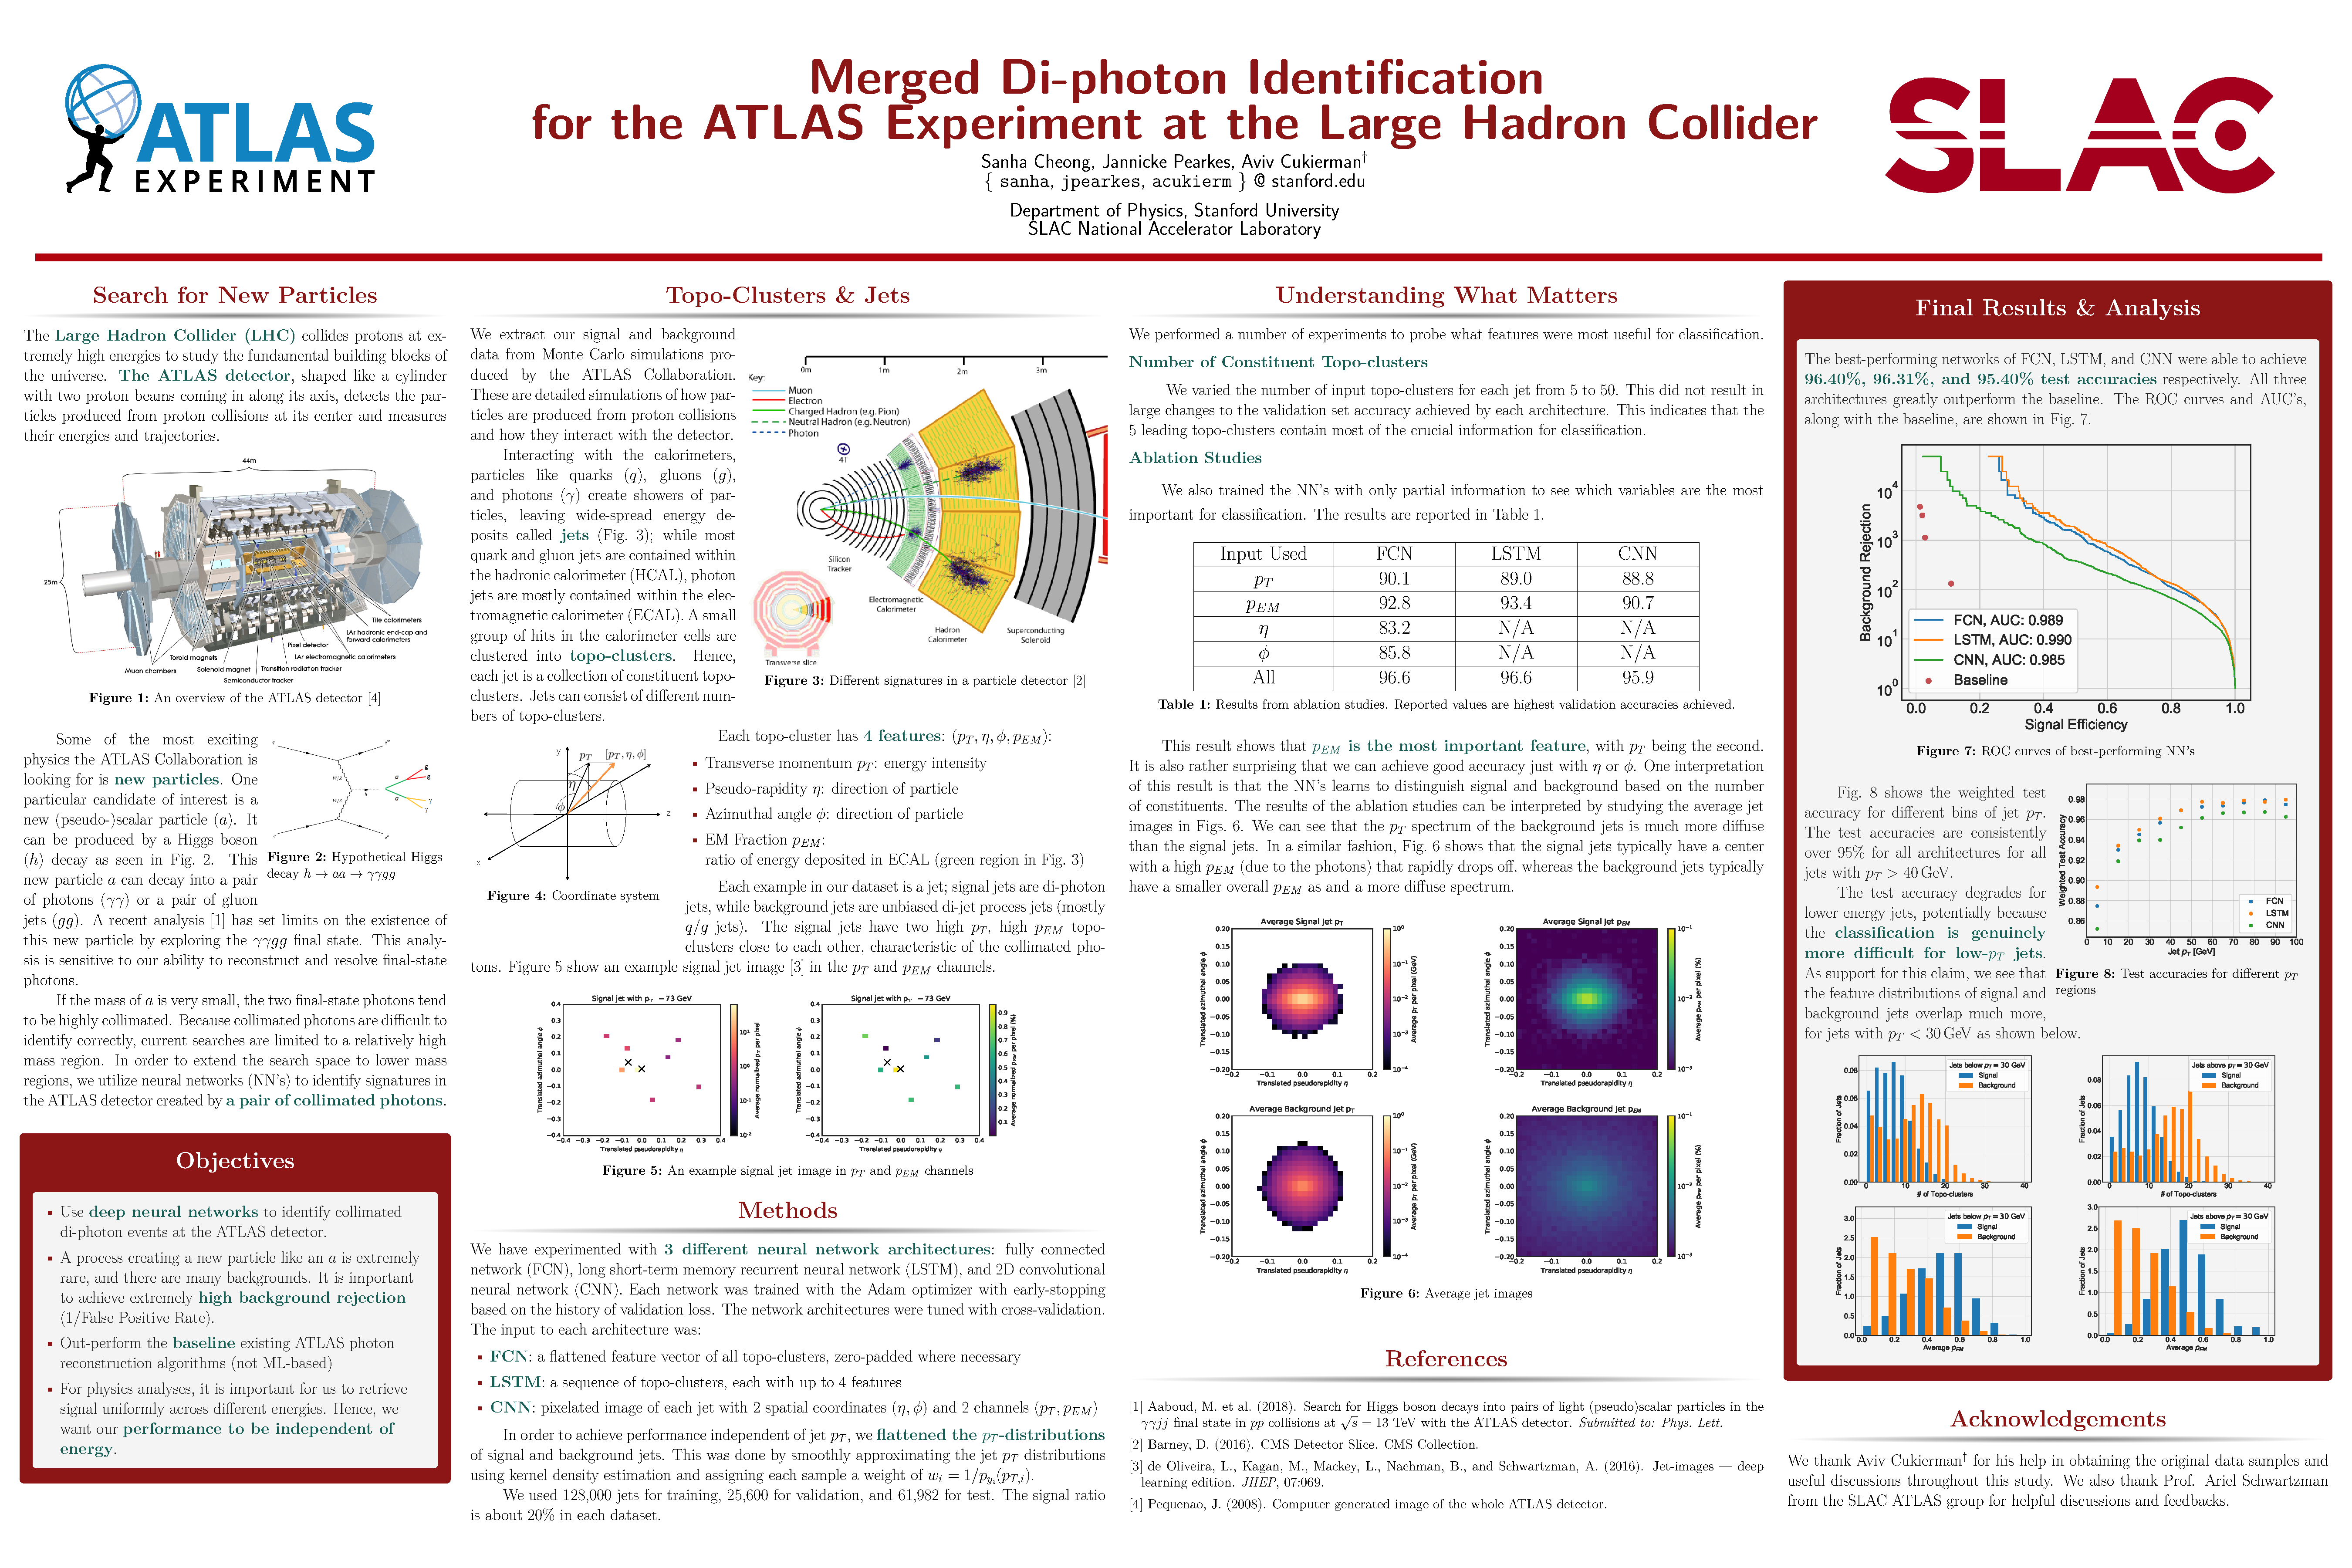
\includegraphics[width=0.8\textwidth]{./cs231n_project_poster.pdf}
            \caption{CS 231N project poster using this template}
            \label{fig:roc_architectures}
        \end{figure}
        
        The \texttt{.pdf} file is also included in the repository.
        
        \hspace{1cm}Feel free to use this template for \emphg{your own posters}.
		
	\end{alertblock}
	
	\begin{block}{Acknowledgements}
		\textsuperscript{$*$}, \textsuperscript{$\dagger$} Surprise, they are all the same person.
	\end{block}
\end{column}

\begin{column}{\sepwid}\end{column}

\end{columns}
\end{frame}
\end{document}